\documentclass[11pt, a4paper]{report}
\usepackage[utf8]{inputenc}%codification of the document
\usepackage[french]{babel}
\usepackage{geometry}
\usepackage{times}
\usepackage{graphicx}
\usepackage{multicol}
\usepackage{float}
\usepackage{subcaption}
\usepackage{comment}
\usepackage{hyperref}
\usepackage{listings}
\usepackage{color}

\definecolor{lightgray}{rgb}{.98,.98,.98}
\definecolor{darkgray}{rgb}{.4,.4,.4}
\definecolor{blue}{rgb}{0.5, 0.2, 0.82}
\definecolor{purple}{rgb}{0.7, 0, 0.6}

\lstdefinelanguage{JavaScript}{
	keywords={typeof, new, true, false, catch, function, return, null, catch, switch, var, if, in, while, do, else, case, break},
	keywordstyle=\color{blue}\bfseries,
	ndkeywords={class, export, boolean, throw, implements, import, this},
	ndkeywordstyle=\color{darkgray}\bfseries,
	identifierstyle=\color{black},
	sensitive=false,
	comment=[l]{//},
	morecomment=[s]{/*}{*/},
	commentstyle=\color{blue}\ttfamily,
	stringstyle=\color{purple}\ttfamily,
	morestring=[b]',
	morestring=[b]"
}

\lstset{
	language=JavaScript,
	backgroundcolor=\color{lightgray},
	extendedchars=true,
	basicstyle=\footnotesize\ttfamily,
	showstringspaces=false,
	showspaces=false,
	numbers=left,
	numberstyle=\footnotesize,
	numbersep=9pt,
	tabsize=2,
	breaklines=true,
	showtabs=false,
	captionpos=b
}



\begin{document}
	\pagenumbering{roman}
	\begin{titlepage}
		\begin{center}
			
			\vspace*{1cm}
			
			\begin{figure}[h]
				\centering
				
\includegraphics[width=0.4\textwidth]{images/LOGO_Polytech-lille.jpg}
				\hspace{2cm}
				
\includegraphics[width=0.4\textwidth]{images/logo_ulille_transparent.png}
			\end{figure}
			
			\vspace*{2cm}
			
			\rule{1\textwidth}{.8pt}
			
			\LARGE{\textsc{Projet tutoré de Structures de Données \\-\\ Graphes et Combinatoires}}
			
			\vspace*{1cm}
			
			\LARGE{\textsc{Problème du flot maximum}}
			\vspace*{1cm}
			
			\small{IS2A3 - Lundi 31 mai 2021}
			
			\vspace*{0.5cm}
			\rule{1\textwidth}{.10pt}
		
			\vspace*{2.352cm}
			
			\large{\textit{Encadrante :} Clarisse DHAENENS}
			
			\vspace*{0.1cm}	        
			
			\large{\textit{Auteurs :} Badmavasan KIROUCHENASSAMY\\Caroline SCHMID} 
			
			
			
			
		\end{center}
		
	\end{titlepage}
	
	
	%\setcounter{tocdepth}{2}
	\tableofcontents
	
	
	\chapter{Contexte du projet}
	\pagenumbering{arabic}
	Pour résoudre un problème de flot maximum, plusieurs algorithmes peuvent être mis en œuvre. Nous étudions ici la mise en place de l'algorithme de \textbf{DINIC} ainsi que les structures de données nécessaires et l'arborescence des fichiers.
	
	Le problème de flot maximum consiste en trouver le flot le plus élevé que l'on puisse faire passer dans un Réseau en respectant les capacités de chaque arc, soit le flot maximum que l'on puisse faire passer par chaque arc.
	
	L'algorithme de \textbf{DINIC} permet, à partir d'un flot initial, de rechercher une chaîne améliorante dans un réseau de façon à construire un flot de valeur supérieure. En réitérant cette opération un certain nombre de fois, le flot que l'on obtient devient maximum. L'algrithme prend en paramètre un graphe d'écart, il faut donc trnsformer le réseau du problème de flot maximum en un graphe d'écart pour trouver le flot maximum et revenir à un réseau répondant au problème posé.
	
	On considère que le flot initial est de 0 et que les sommets sont au nombre de $n$ et numérotés de $1$ à $n$.
	
	
	
	\chapter{Analyse}
	\section{Représentation des données}
	La chaîne améliorante de l'algorithme de \textbf{DINIC} est la chaine du plus court chemin en nombre d'arcs et sera trouvée donc par l'algorithme de parcours en largeur. Étant donné que ce dernier algorithme génère l'arborescence donnant le plus court chemin en nombre d'arc, on l'utilise pour trouver la chaîne améliorante de l'algorithme de \textbf{DINIC}.
	
	L’algorithme de parcours en largeur est un algorithme parcourant le graphe par couches. Les sommets de la couche $n$ sont à une distance $n$ du sommet source. L’exploration commence donc par la source, puis ses successeurs, puis les successeurs de ses successeurs, ... jusqu’à explorer le sommet puits et on sait alors que l’on peut s’arrêter. Grâce à un tableau répertoriant les prédécesseurs des sommets marqués (par convention, le sommet prédécesseur du sommet source est lui-même), on peut retrouver le chemin le plus court en nombre d'arcs menant d’un sommet à un autre (ici, menant du sommet source au sommet puits).
	
	Voici le déroulement de l'algorithme de \textbf{DINIC} sur un réseau à 5 sommets et 7 arcs :
	\begin{enumerate}
		\item \verb|Réseau :|\\
	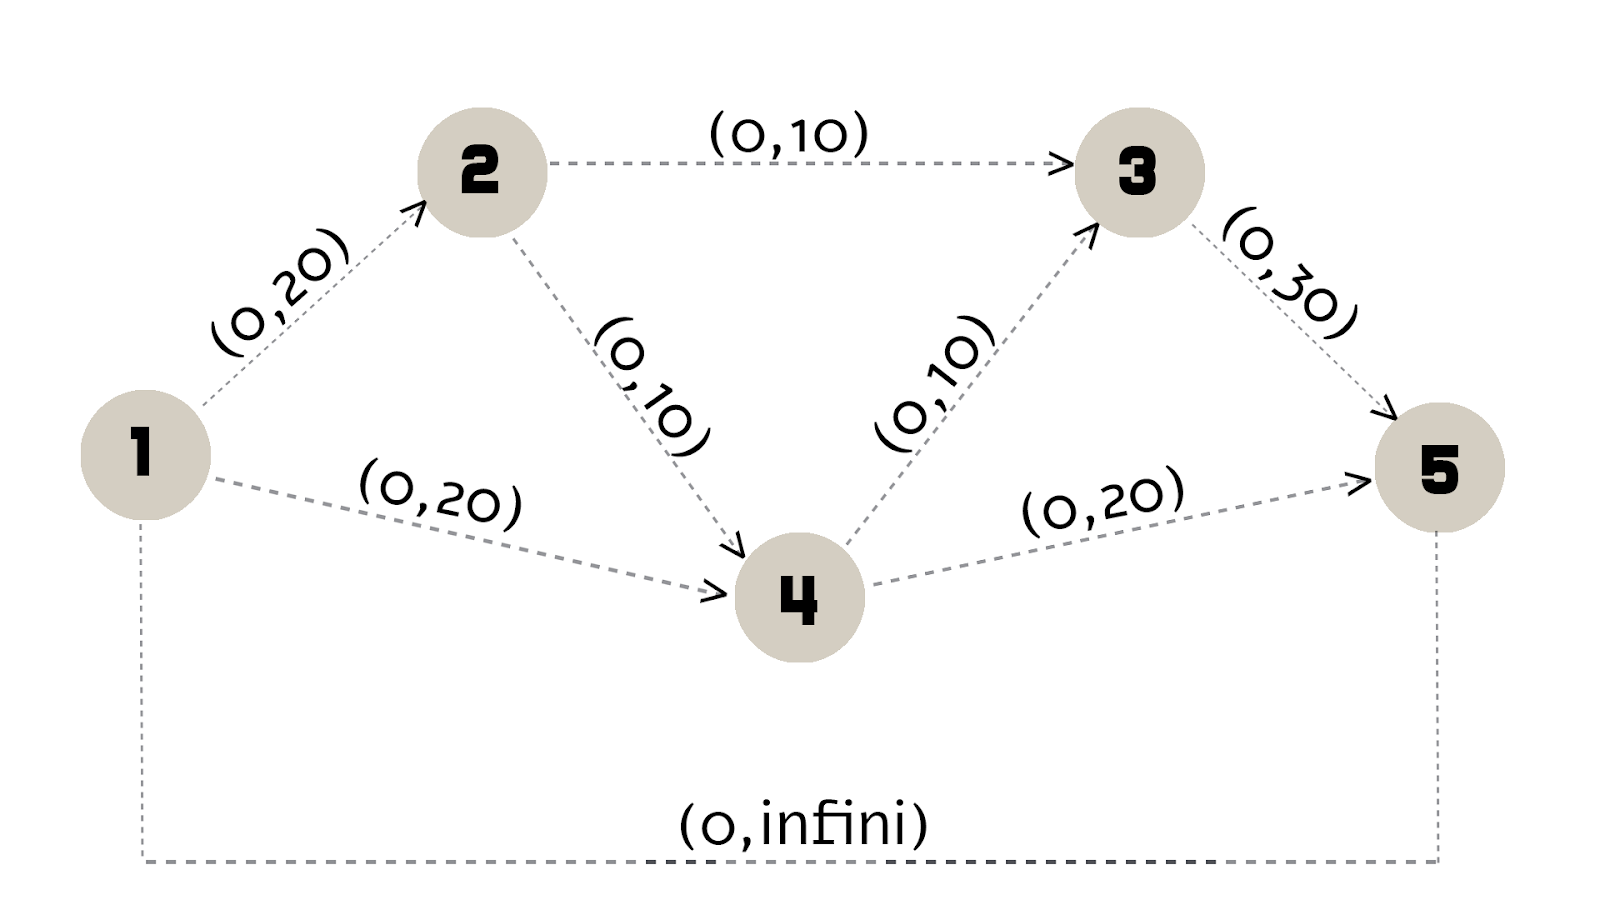
\includegraphics[width=0.7\textwidth]{images/R1.png}\\
	\pagebreak
		\item \verb|Graphe d'Écart :|\\
	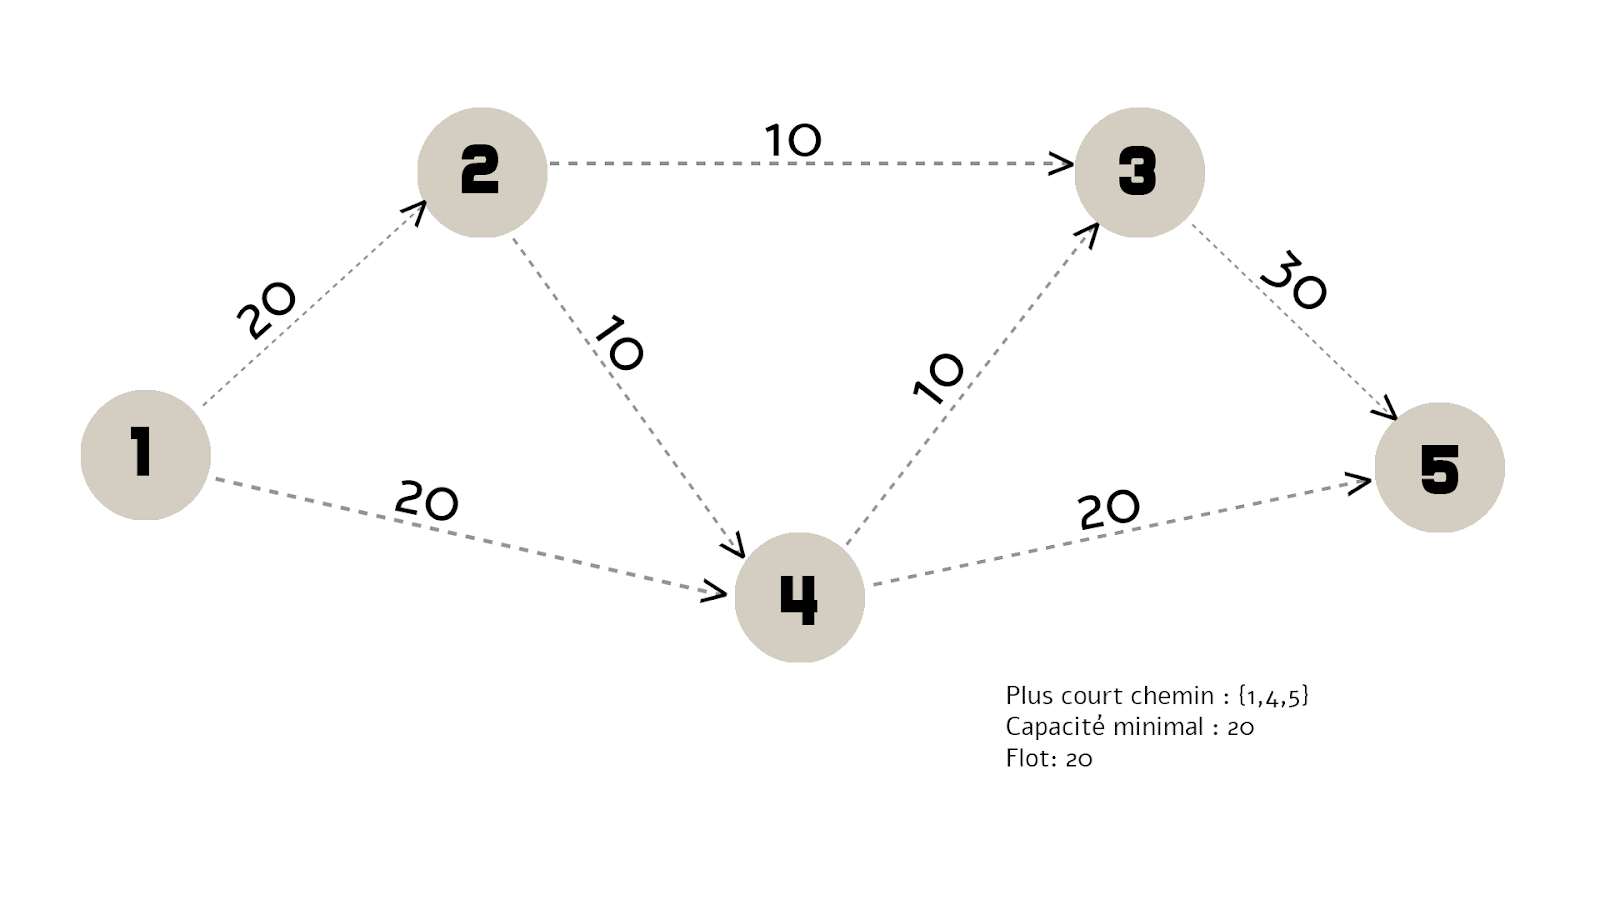
\includegraphics[width=0.7\textwidth]{images/GE1.png}\\
		\item \verb|Graphe d'Écart :|\\
	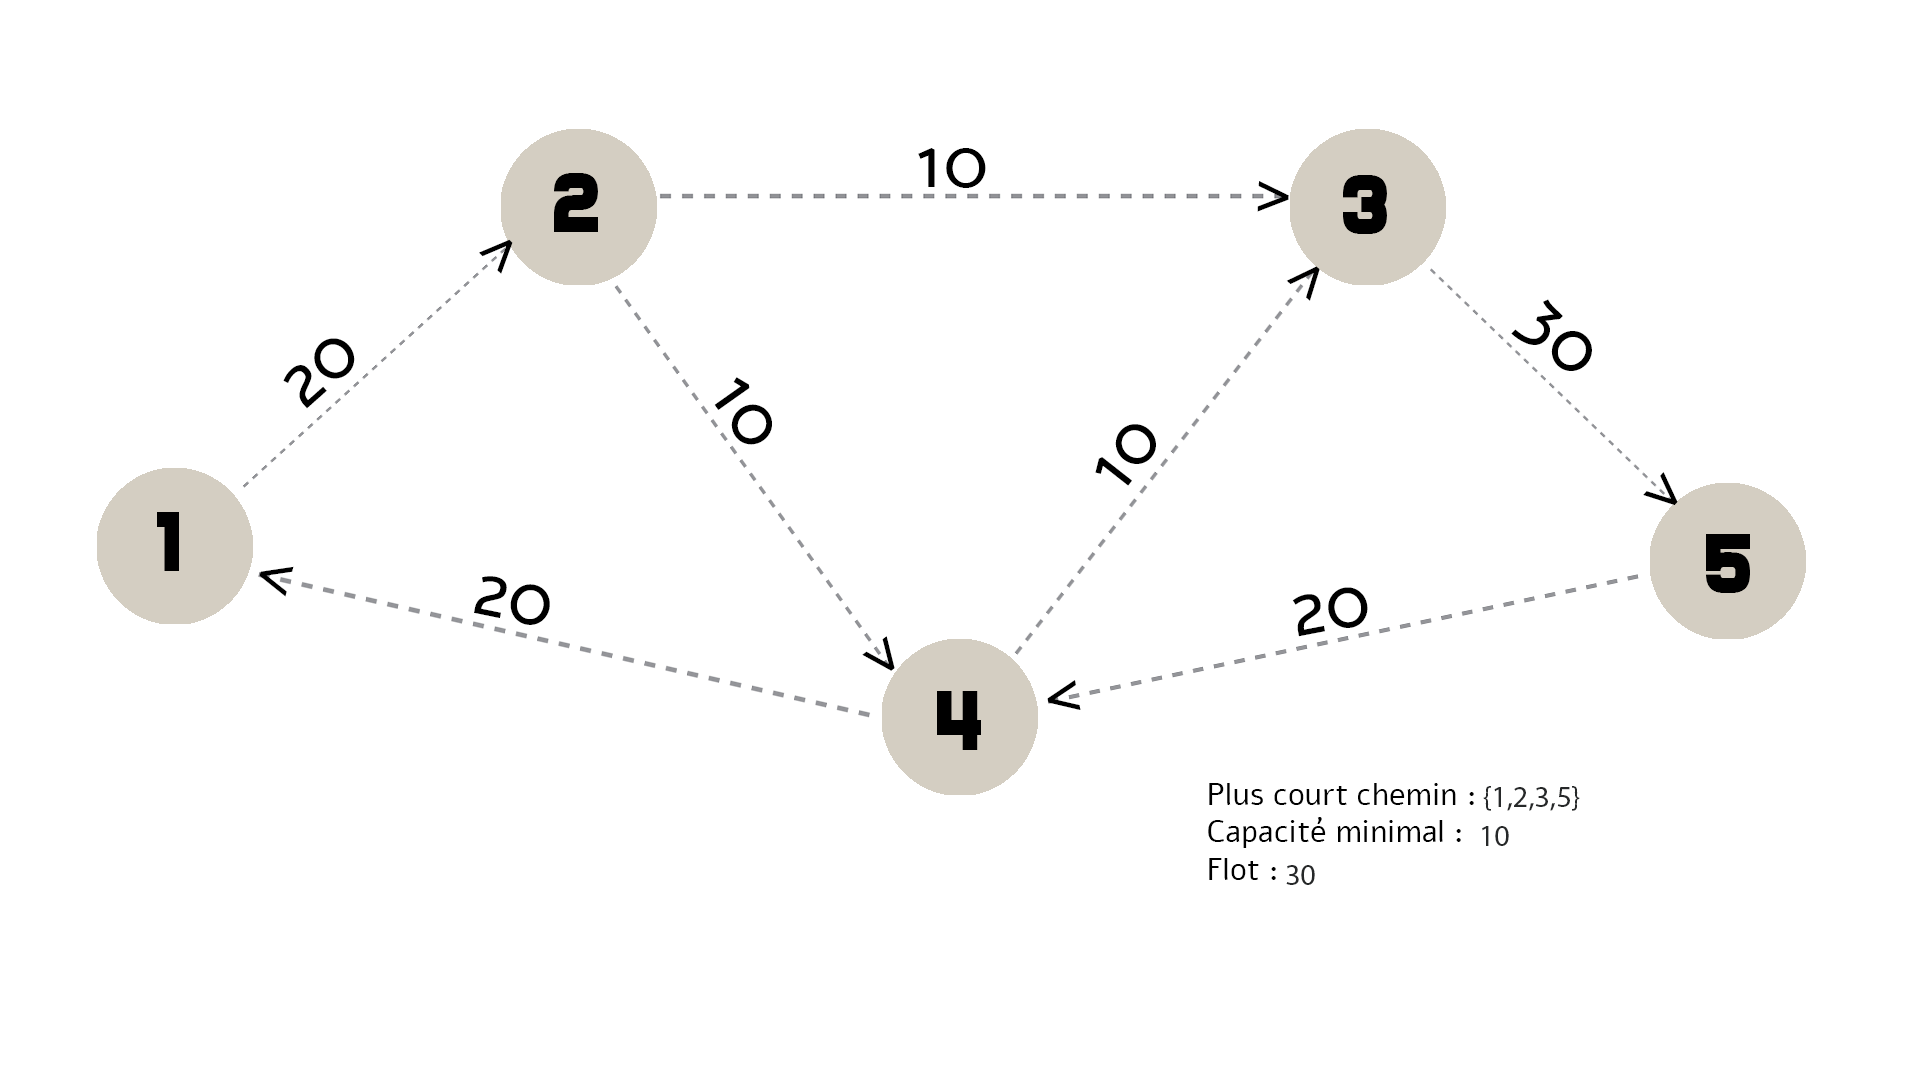
\includegraphics[width=0.7\textwidth]{images/GE2.png}\\
		\item \verb|Graphe d'Écart :|\\
	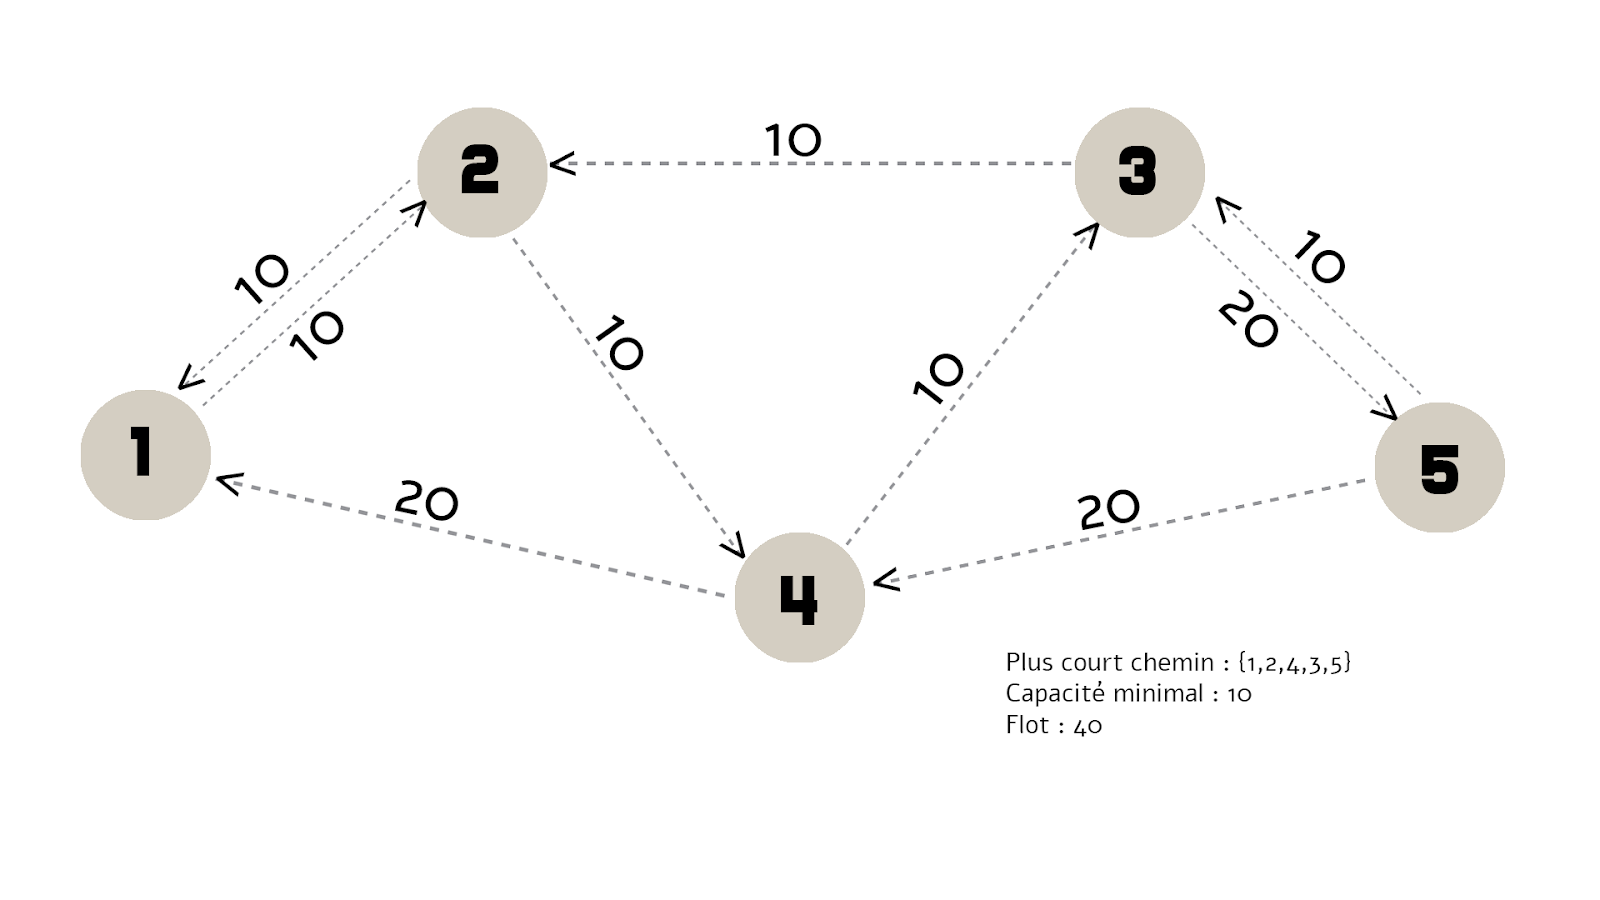
\includegraphics[width=0.7\textwidth]{images/GE3.png}\\
	\pagebreak
		\item \verb|Graphe d'Écart :|\\
	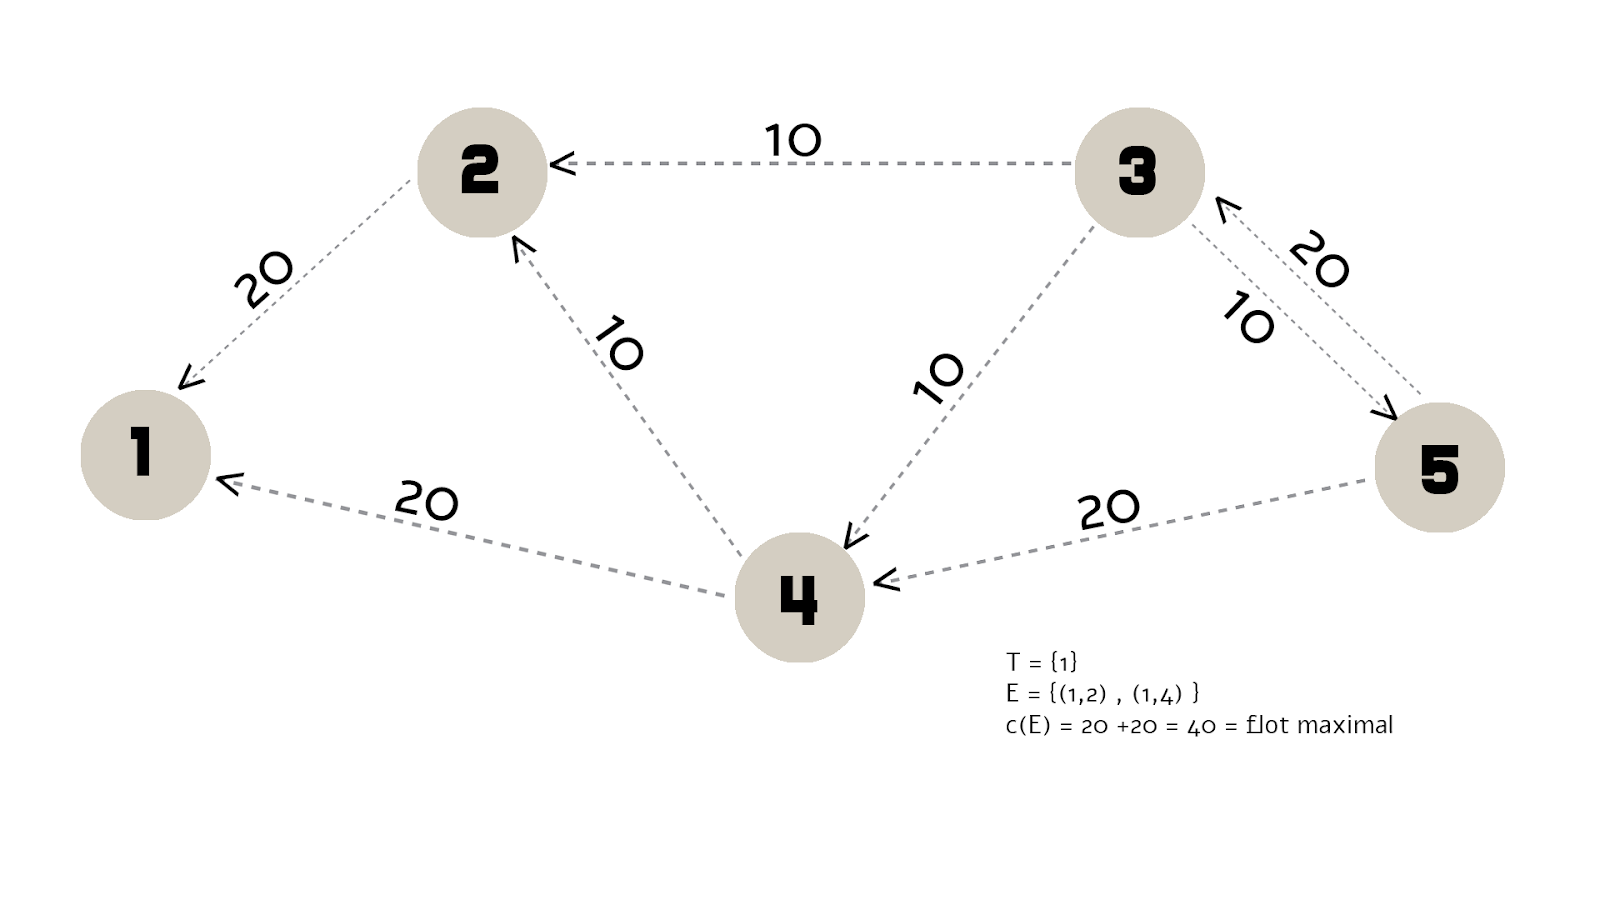
\includegraphics[width=0.7\textwidth]{images/GE4.png}\\
		\item \verb|Réseau :|\\
	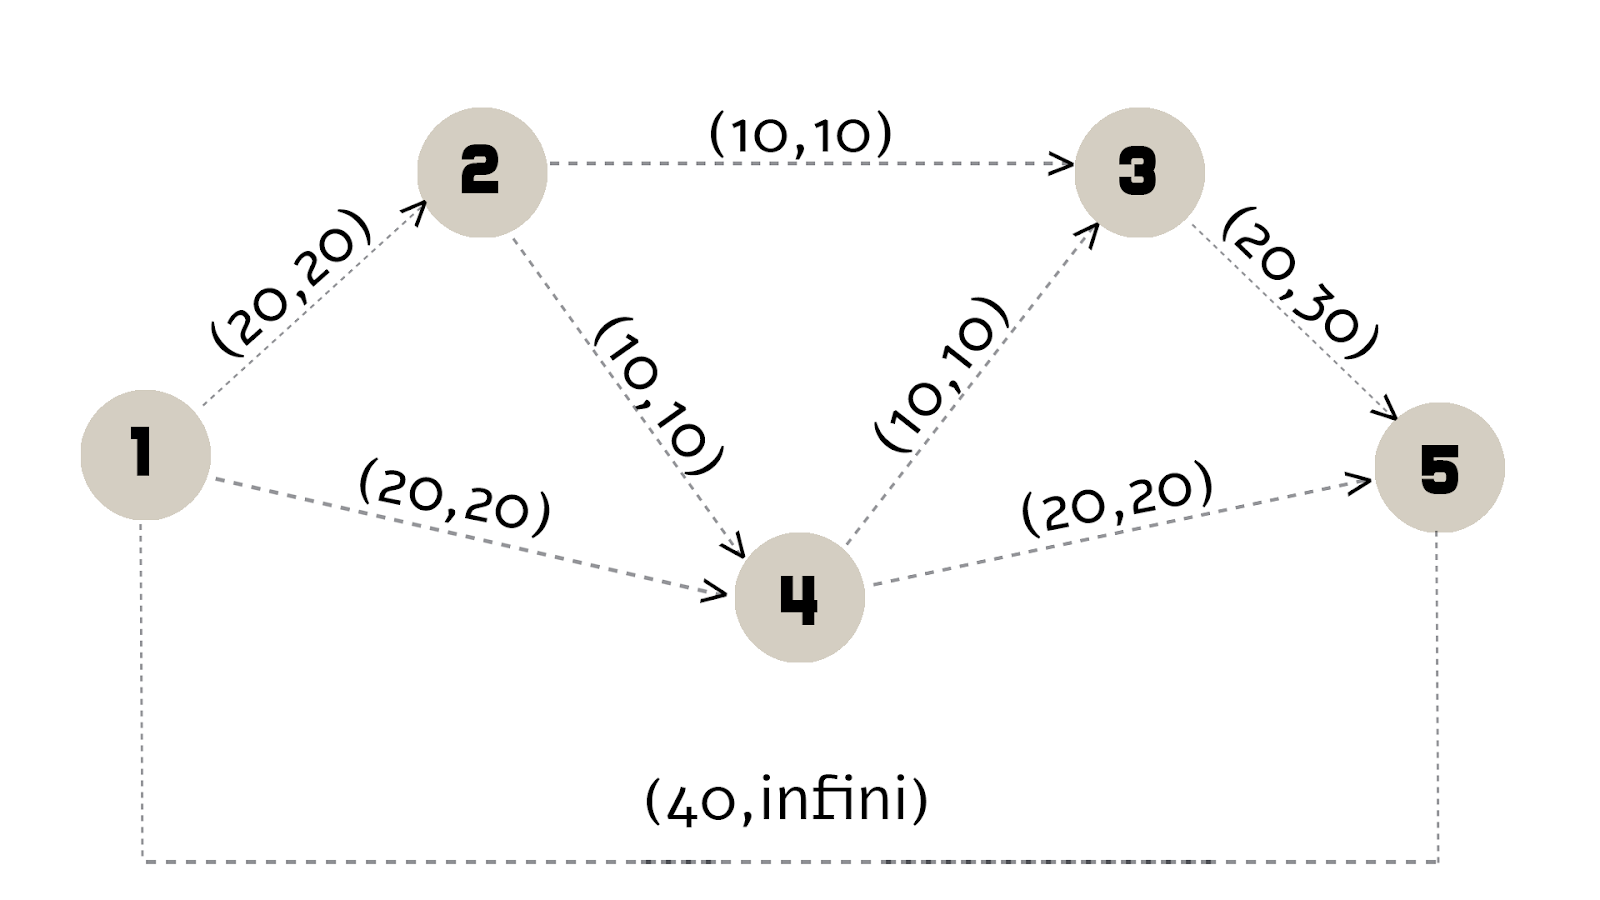
\includegraphics[width=0.7\textwidth]{images/R2.png}\\
	\end{enumerate}
	
	Par convention, un graphe est constitué de $n$ sommets et $m$ arcs. On utilisera donc ces notations pour alléger le texte.
	
	Pour représenter le réseau, on voit trois structures de données possibles :
	\begin{enumerate}
		\item une matrice d'incidence :
		
		Un tableau de tableaux : chaque case du premier tableau est elle-même un tableau. les sommets sont représentés en lignes et les arcs en colonnes. La case est à $0$ si le sommet n'est pas incident à l'arc, $1$ s'il est source de l'arc et $-1$ s'il est destination de l'arc.\\
		\includegraphics[width=0.7\textwidth]{images/Matrice_d-incidence.extension}\\
		
		\item un tableau sommets - successeurs :
		
		Deux tableaux.Le premier tableau de la longueur du nombre d'arc est un tableau de pointeurs pointant vers le premier sommet successeur dans le second tableau. Le second tableau, de la longueur du nombre d'arcs, représente les successeurs des sommets du premier tableau. Les successeurs d'un même sommet sont contigus dans le second tableau.\\
		\includegraphics[width=0.7\textwidth]{images/Tableau_sommets-successeurs.extension}\\
		
		\item un tableau de listes de successeurs :
		
		Un tableau de listes de successeurs. Chaque case contient une liste. La tête de la liste indique quel est le sommet source et les maillons de la liste sont les successeurs de ce sommet source.\\
		\includegraphics[width=0.7\textwidth]{images/Tableau_de_listes_de_successeurs.extension}\\
		
	\end{enumerate}
	
    Comparons les avantages des trois structures de données sur 3 critères : le coût de stockage en mémoire, le coût de traitement en accès au successeur d'un sommet donné et finalement l'ajout et la suppression d'un successeur d'un sommet donné.
    
    \begin{center}
        \begin{tabular}{ | c | c | c | c | } 
            \hline
            & Matrice d'incidence & Tableau sommets - successeurs & Tableau de listes de successeurs \\
            \hline
            Coût de stockage en mémoire & La dimension de la matrice est de $n·m$. L'initialisation du tableau occupe une taille de $n·m$, donc la complexité en coût mémoire vaut $(n·m).sizeof(int)$. & La complexité en coût mémoire de cette structure de donnée est simplement de $n+m$. & Le tableau initial est de taille $n$ et il y a $m$ maillons répartis dans les différentes listes du tableau. Ces structures sont allouées dynamiquement. La complexité en coût mémoire est de nouveau de $n+m$.\\
            \hline
            Coût de traitement en accès au successeur & Il faut parcourir la matrice afin de trouver les successeurs d'un sommet vu que c'est une matrice d'incidence donc on ne peut pas se concentrer sur une seule ligne ou colonne. La complexité est donc de $O(n·m)$. & On a directement l'indice dans le tableau de successeurs en fonction du tableau de sommets. Donc on n'a pas vraiment de traitement à effectuer. La complexité est donc de $O(m)$. & On a une listechaînée donc il y a le coût de parcours des maillons. La complexité est donc de $O(m)$.\\
            \hline
            Ajout et la suppression d'un successeur & Il faut redimensionner une matrice à 2 dimensions et donc réalouer plus ou moins de mémoire et déplacer les données étant donné qu'elles sont stockées dans des cases contigues (principe du tableau). La complexité et en $O(n·m)$. & Le second tableau, de successeurs, doit être redimensionné et donc il faut potentiellement déplacer le tableau. La complexité de cette opération est en $O(m)$. & L'ajout ou la suppression d'un maillon dans une liste a un coût constant et donc négligeable. Sa complexité est en $O(1)$.\\
            \hline
        \end{tabular}
    \end{center}
    La structure de données correspondant le plus aux opérations que l'algorithme de \textbf{DINIC} nécessite est la structure de données en tableau de listes de successeurs étant donné que pour le coût de stockage en mémoire et pour le coût de traitement en accès au successeur, la complexité est la même entre cette solution et le tableau sommets - successeurs et qu'elle a une complexité plus faible en ajout et la suppression d'un successeur que cette dernière. La matrice d'incidence à une complexité largement moins bonne que celle du tableau de listes de successeurs sur les différents critères.
    
    Pour réduir le nombre d'ajout et de suppressions d'arcs dans le graphe d'écart lors de ses mises à jour entre deux itérations de \textbf{DINIC}, on pourrait, lors de la création du graphe à partir du réseau, créer pour chaque sommet dans le graphe un arc avec le flot égalant la capacité de l'arc du graphe et un arc inverse de flot nul. Ça permettrait d'utiliser les arcs déjà construits et ne pas ajouter de nouvel arc ou en retirer un de flot nul.
    
    Nous n'appliquerons pas cette idée car elle permet d'économiser un peu d'espace mémoire. L'espace économisé n'est pas nécessairement important mais il devient significatif lorsque le nombre d'arcs devient grand car on passe de $m$ arcs à $2m$ arcs. On notera que cette solution aurait pu être appliquée au tableau sommets - successeurs et il n'y aurait plus eu d'avantages à utiliser la soulution retenue plutôt que cette structure de données avec $2m$ arcs pour les deux structures de données.
    
	\section{Implémentation de la structure de données choisie}
	
	Pour dérouler l'algorithme de \textbf{DINIC} et trouver le flot maximum du réseau donné, on utilisera 4 structures de données : 
	\begin{enumerate}
		\item Une liste, et ses maillons, représentant les successeurs d'un sommet dans le réseau (listes constituant le tableau de de listes de successeurs).
		\item Une liste, et ses maillons, représentant les successeurs d'un sommet dans le graphe d'écart (listes constituant le tableau de de listes de successeurs).
		\item Une liste, et ses maillons, représentant les sommets constituant le plus court chemin en nombre d'arcs permettant d'améliorer le flot d'un graphe donné.
		\item Une file permettant de trouver le plus court chemin en nombre d'arcs dans un graphe donné.
	\end{enumerate}
	
	Voici le code $C$ décrivant ces structures de données :
	\lstset{language=C}
	\begin{lstlisting}
        /* Réseau */
        
        struct maillon_graph_reseau {
            int id;
            int flot;
            int capacite;
            struct maillon_graph_reseau* next;
        };

        struct liste_graph_reseau {
            int id;
            struct maillon_graph_reseau* head;
        };
        
        
        
        /* Graphe Écart */
        
        struct maillon_graph_ecart {
            int id;
            int flot_entrant;
            struct maillon_graph_ecart* next;
        };

        struct liste_graph_ecart {
            int id;
            struct maillon_graph_ecart* head;
        };
        
        
        
        /* Chemin */
        
        struct maillon_chemin {
            int id;
            int capacite_residual;
            struct maillon_chemin * next;
        };
        
        struct liste_chemin {
            struct maillon_chemin * head;
        };
        
        
        
        /* File */
        
        struct file {
            int* tab;
            int taille;
            int read_end;
            int write_end;
            int n;
        };
	\end{lstlisting}
	
	Lorsqu'un maillon est le dernier de la liste, il pointe vers un pointeur null de son type :
	
	\lstset{language=C}
	\begin{lstlisting}
        /* Réseau */
        
        #define NIL_lr (struct liste_graph_reseau*) 0
        #define NIL_mr (struct maillon_graph_reseau*) 0
        
        
        
        /* Graphe Écart */
        
        #define NIL_lge (struct liste_graph_ecart *) 0
        #define NIL_mge (struct maillon_graph_ecart *) 0
        
        
        
        /* Chemin */
        
        #define NIL_lc (struct liste_chemin *) 0
        #define NIL_mc (struct maillon_chemin *) 0
	\end{lstlisting}
	
	De manière schématique, les structures de données ressembleraient donc à :
	\begin{itemize}
        \item Réseau :\\
		\includegraphics[width=0.7\textwidth]{images/}\\
        \item Graphe Écart :\\
		\includegraphics[width=0.7\textwidth]{images/}\\
        \item Chemin :\\
		\includegraphics[width=0.7\textwidth]{images/}\\
        \item File :\\
		\includegraphics[width=0.7\textwidth]{images/}\\
	\end{itemize}
	
	L'arborescence des fichiers est la suivante :
	
	\begin{figure}[H]
		\captionsetup{justification=centering}
		\centering
		\includegraphics[width=0.6\textwidth]{images/ants2m.png}
	\end{figure}
	
	La descritpion de la file ainsi que les déclarations des fonctions applicables dessus se trouvent dans le ficher \verb|File.h| et ses fonctions sont décrites dans le fichier \verb|File.c|.
	
	Le réseau et le graphe d'écart sont tout deux des graphes et le chemin est construit à partir d'un graphe donc les fonctions dépendant de ces 3 structures de données sont contenues dans le ficher \verb|Graph.c|. Ce dernier importe 4 fichiers d'entête : \verb|GraphReseau.h|, \verb|GraphEcart.h| et \verb|Chemin.h| contenant la description des structures de données respectives. Le 4^{ième} fichier importé est \verb|Graph.c|, contenant la déclaration des fonctions produites dans le fichier \verb|Graph.c|.
	
	Enfin, \verb|Dinic.h| contient la signature de la fonction programmée dans le fichier \verb|Dinic.c| et \verb|main.c| fait tourner le programme et maximise le flot du réseau donné en paramètres.
	
	Ainsi, la File est importée dans le Chemin pour permettre de trouver le plus court chemin, le Chemin, le Graphe Écart et le Réseau sont importés dans le Graphe, le Graphe est importé dans Dinic et enfin Dinic est importé dans le main.
	
	\chapter{Mode d'emploi}
	
	L'entrée du programme est un fichier contenant la description d'un réseau au format \textbf{DIMACS}. (des exemples de ce format sont présents dans le dossier $./DIMACS/$ ou encore sur $MOODLE$).
	
	On va donc exécuter notre programme sur ce réseau pour maximiser le flot et obtenir un nouveau fichier $result.txt$ en sortie, contenant la description du réseau de flot maximum ainsi que le flot maximum final.
	
	
	
	
	\begin{figure}[H]
		\centering
		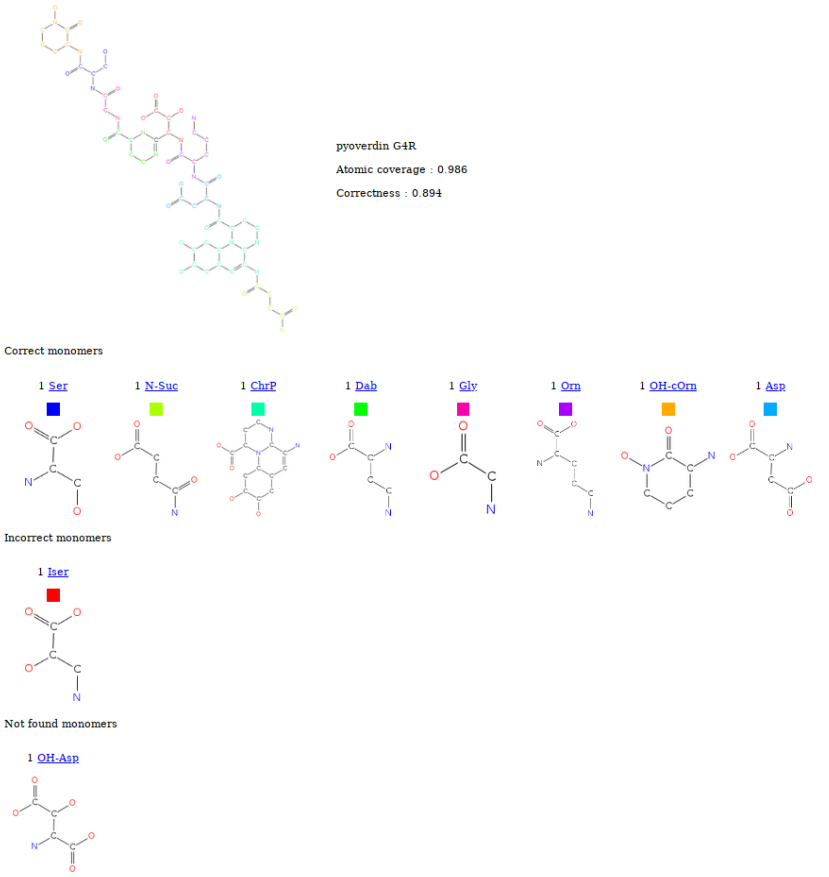
\includegraphics[width=0.9\textwidth]{images/pyoverdin G4R.png}
		\hspace{2cm}
		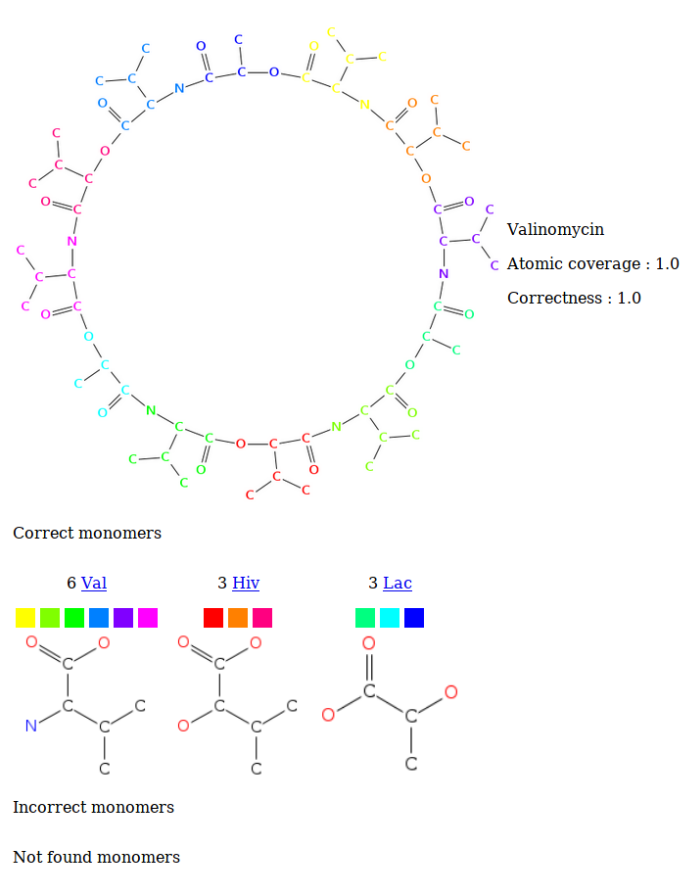
\includegraphics[width=0.5\textwidth]{images/Valinomycin.png}
	\end{figure}
	
	\begin{figure}[H]
		\captionsetup{justification=centering}
		\centering
		\includegraphics[width=0.6\textwidth]{images/ants2m.png}
	\end{figure}
	\vspace{0.000000000001cm}
	\begin{figure}[H]
		\captionsetup{justification=centering}
		\centering
		\includegraphics[width=0.6\textwidth]{images/ants2m-D.png}
	\end{figure}
	
	
	\chapter{Description des exemples traités}
	\begin{itemize}
		\item "\verb|.|" : Les Smiles contenant des points sont plusieurs polymères, il faut donc couper au niveau du point et traîter séparément chaque polymère (ex:
		\\"\verb|CC(C)(C)OC(=O)N[C@H](CC1=CC=C(C=C1)I)C(=O)=C.CC(C)(C)|\\\verb|OC(=O)N[C@@H](CC1=CC=C(C=C1)I)C(=O)=C|" devient \\"\verb|CC(C)(C)OC(=O)N[C@H](CC1=CC=C(C=C1)I)C(=O)=C|" et\\  "\verb|CC(C)(C)OC(=O)N[C@@H](CC1=CC=C(C=C1)I)C(=O)=C|" [ici, les deux polymères sont l'isomère l'un de l'autre]).
	\end{itemize}

	\chapter{Pseudo-Code}
	%\lstset{language=C}
	\begin{lstlisting}
		Coverage :
		0.0 -> 195
		0.1 -> 0
		0.2 -> 1
		0.3 -> 8
		0.4 -> 1699
		0.5 -> 315
		0.6 -> 2375
		0.7 -> 25427
		0.8 -> 139092
		0.9 -> 207199
		1.0 -> 126079
		NaN -> 14
	\end{lstlisting}
	
	
	\chapter*{Conclusion}
	\pagenumbering{Alph}
	
	\begin{figure}[H]
		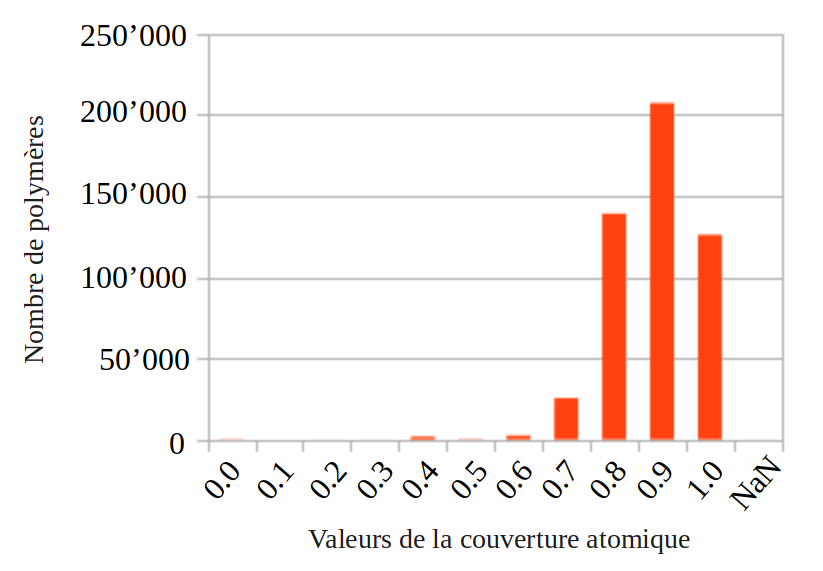
\includegraphics[width=0.8\textwidth]{./images/ACs2m.png}
	\end{figure}
	La majorité des polymères sont recouverts à plus de 70\% et le taux de couverture de la majorité des polymères est de 0.9.
	
	
	\chapter*{Bilan personnel}
	
	
\end{document}
